\documentclass[11pt, a4paper, pdf]{article}
\newcounter{minitocdepth}
\newcounter{chapter}
\newcommand{\chaptername}{}

\include{estil-llibre}

\renewcommand{\hot}[1][]{
	\ifthenelse{\equal{#1}{}}{$\mathbf{\bigstar}$ LLIBRE $\mathbf{\bigstar}$: }{\myrepeat{#1}{$\mathbf{\bigstar}$}}
}
 \renewcommand{\normalsize}{\fontsize{10.5}{11.2}\selectfont}
 
 \fancypagestyle{blocfancy}{
 	\pagestyle{fancy}% Duplicate fancy page style
 	\fancyhead{} % clear all header fields
 	\fancyhead[RE,LO]{\textit{IES Binissalem. Apunts de vectors en el pla}}
 	\fancyhead[LE,RO]{\bfseries\large\thepage}
 }
 
\begin{document}
\pagestyle{blocfancy}
\setcounter{myenumi}{0}
 
 \begin{center}
 {\Large  \textbf{Apunts de vectors en el pla}}
 \end{center}
 \begin{blueshaded}
 	Les diferents magnituds en la naturalesa es classifiquen en \textbf{escalars i vectorials}. Una magnitud és vectorial si depèn de la direcció.
 	\begin{center}
 		\begin{tabular}{p{0.35\textwidth} | p{0.35\textwidth}}
 			\textbf{Magnituds escalars} & \textbf{Magnituds vectorials} \\ \hline
 			Temps       & Velocitat \\
 			Temperatura & Acceleració \\
 			Volum       & Força \\
 			$\cdots$   & $\cdots$ 
 		\end{tabular}
 	\end{center}
 	
 	Un vector queda determinat per dos punts $A$ \textbf{origen} i $B$ l'\textbf{extrem}. El \textbf{mòdul} és la llargària del vector o la distància entre $A$ i $B$. La \textbf{direcció} és la de la recta que passa per $A$ i $B$. Cada direcció té dos \textbf{sentits}.
 \end{blueshaded}
 

\begin{mylist}
	
	\item 
	
	La figura ABCDEF és un hexàgon. Compara el mòdul, la direcció i el sentit dels següents parells de vectors.
	
	\begin{minipage}{0.6\textwidth}
		\begin{tasks} 
			\task $\overrightarrow{AB}$ i	$\overrightarrow{BC}$
			\task $\overrightarrow{FE}$ i	$\overrightarrow{BC}$
			\task $\overrightarrow{BM}$ i	$\overrightarrow{DE}$
			\task $\overrightarrow{OS}$ i	$\overrightarrow{OE}$
		\end{tasks}
	\end{minipage}
	\begin{minipage}{0.34\textwidth} 
		\begin{center}
			\vspace{-0.25cm}
			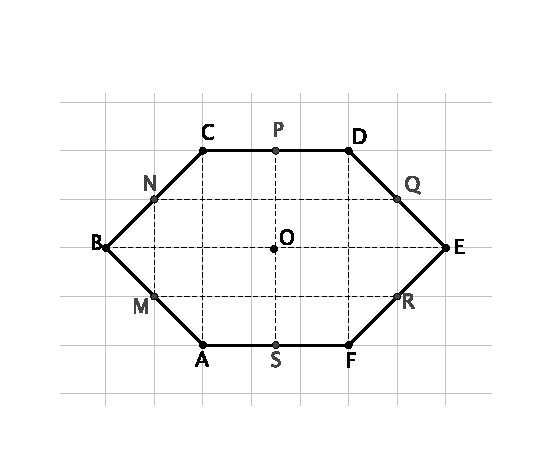
\includegraphics[width=0.9\textwidth]{img2/chap-vect-hexagon}
		\end{center}
	\end{minipage}
	
	
\end{mylist}

 
 \vspace{-1cm}
 
 
 %%%%%%%%%%%%%%%%%%%%%%%%%%%%%%%%%%%%%%%%%%%%%%%%%%%%%%%%%%%%%%%%%%%%%%%%%%%%%%%%%%%%%%%%%%%%%%%%%%%%%%%%%%%%%%%%%%%%%%%%%%%%%%%%%%%%%%%%%%%%%%%%
 \section{Vectors fix i lliure}
 \begin{theorybox}
 			\begin{wrapfigure}{R}{0.25\textwidth} 
 		\vspace{-0.5cm}
 		\begin{center}
 			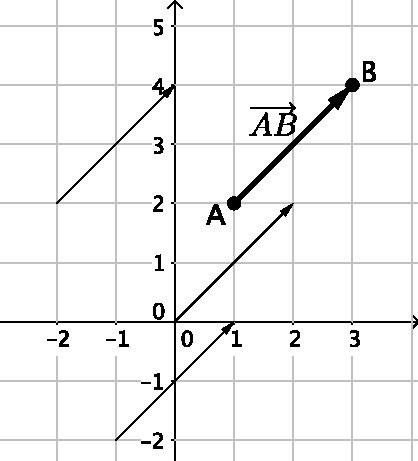
\includegraphics[width=0.23\textwidth]{img2/vec-lliure}
 		\end{center}
 	\end{wrapfigure}
 	Per localitzar un punt $P$ donam dues coordenades $(P_x, P_y)$ que corresponen a les projeccions sobre els eixos $OX$, $OY$ respectivament.
 	
 	Definim un \textbf{vector fix} d'origen en el punt A i extrem en el punt B com el segment orientat que va de A cap a B. 
 	
 	Les components del vector s'obtenen de ``extrem -- origen" 
 	
 	$\overrightarrow{AB}=B-A=(B_x-A_x, B_y-A_y)$.
 	
 	Si ens donen les components d'un vector $\vvec=(\vx, \vy)$, sense especificar-ne l'origen, vol dir que el podem dibuixar amb l'origen que nosaltres vulguem. El consideram un \textbf{vector lliure}.
 \end{theorybox}

\begin{mylist}
	\item Donats els punts $P=\left(2,\, \; 2\right)$, $Q=\left(1,\, \; 0\right)$ i $\, R=\left(-2,\, \; 3\right)$ calcula els vectors
	\begin{tasks}(4)
		\task $\overrightarrow{QP}$    
		\task $\overrightarrow{PQ}$
		\task $\overrightarrow{QR}$  
		\task $\overrightarrow{RP}$
	\end{tasks}
	Quina relació existeix entre els vectors $\overrightarrow{QP}$ i $\overrightarrow{PQ}$?
\end{mylist}

\vspace{-0.5cm}

 %%%%%%%%%%%%%%%%%%%%%%%%%%%%%%%%%%%%%%%%%%%%%%%%%%%%%%%%%%%%%%%%%%%%%%%%%%%%%%%%%%%%%%%%%%%%%%%%%%%%%%%%%%%%%%%%%%%%%%%%%%%%%%%%%%%%%%%%%%%%%%%%
 \section{Operacions amb vectors lliures}
 
 \begin{theorybox}
 	Donats els vectors $\vec u=(-2, 5)$ i $\vvec=(3,1)$ es poden realitzar les següents operacions:
 	
 	\begin{itemize}
 		\item \textbf{Multiplicar per un escalar:}  $7 \vec u = 7 (-2, 5) = (-14, 35)$. És un vector que té igual direcció que $\vec u$, mòdul 7 vegades més llarg i igual sentit. Si multiplicam per $-7$, el sentit és l'oposat.
 		
 		\item \textbf{Sumar:} $\vec u + \vvec=(-2, 5)  + (3,1) = (1, 6)$
 		
 		\item \textbf{Restar:} $\vec u - \vvec=(-2, 5)  - (3,1) = (-5, 4)$
 		
 		\item \textbf{Fer una combinació lineal:} $5 \vec u - 2\vvec =5(-2, 5)  - 2(3,1) = (-10, 25)-(6,2)=(-16, 23)$
 	\end{itemize}
 	
 	Si tenim un vector $\vvec=(\vx,\vy)$, definim el \textbf{vector oposat} com $-\vvec=(-\vx, -\vy)$. L'oposat compleix que $\vvec+(-\vvec)=\vec 0$,
 	on hem definit el \textbf{vector zero} com $\vec 0=(0, 0)$.
 	
 		No confondre amb el vector zero  $\vec 0=(0, 0)$ amb el nombre $0$.
 \end{theorybox} 

 
\begin{mylist}
	
	\item Donats els vectors $\vec u$ i $\vvec$ de la figura, calcula les components de: 
	
	 \begin{minipage}{0.6\textwidth}
	 \begin{tasks}
		\task $2\vec u + \vvec$	
		\task $\vec u - \vvec$
		\task $3\vec u + \frac{1}{3} \vvec$
		\task $-\frac{1}{2} \vec u -2 \vvec$
	\end{tasks}
\end{minipage}
\begin{minipage}{0.4\textwidth}
		\begin{center}
			\vspace{-1cm}
			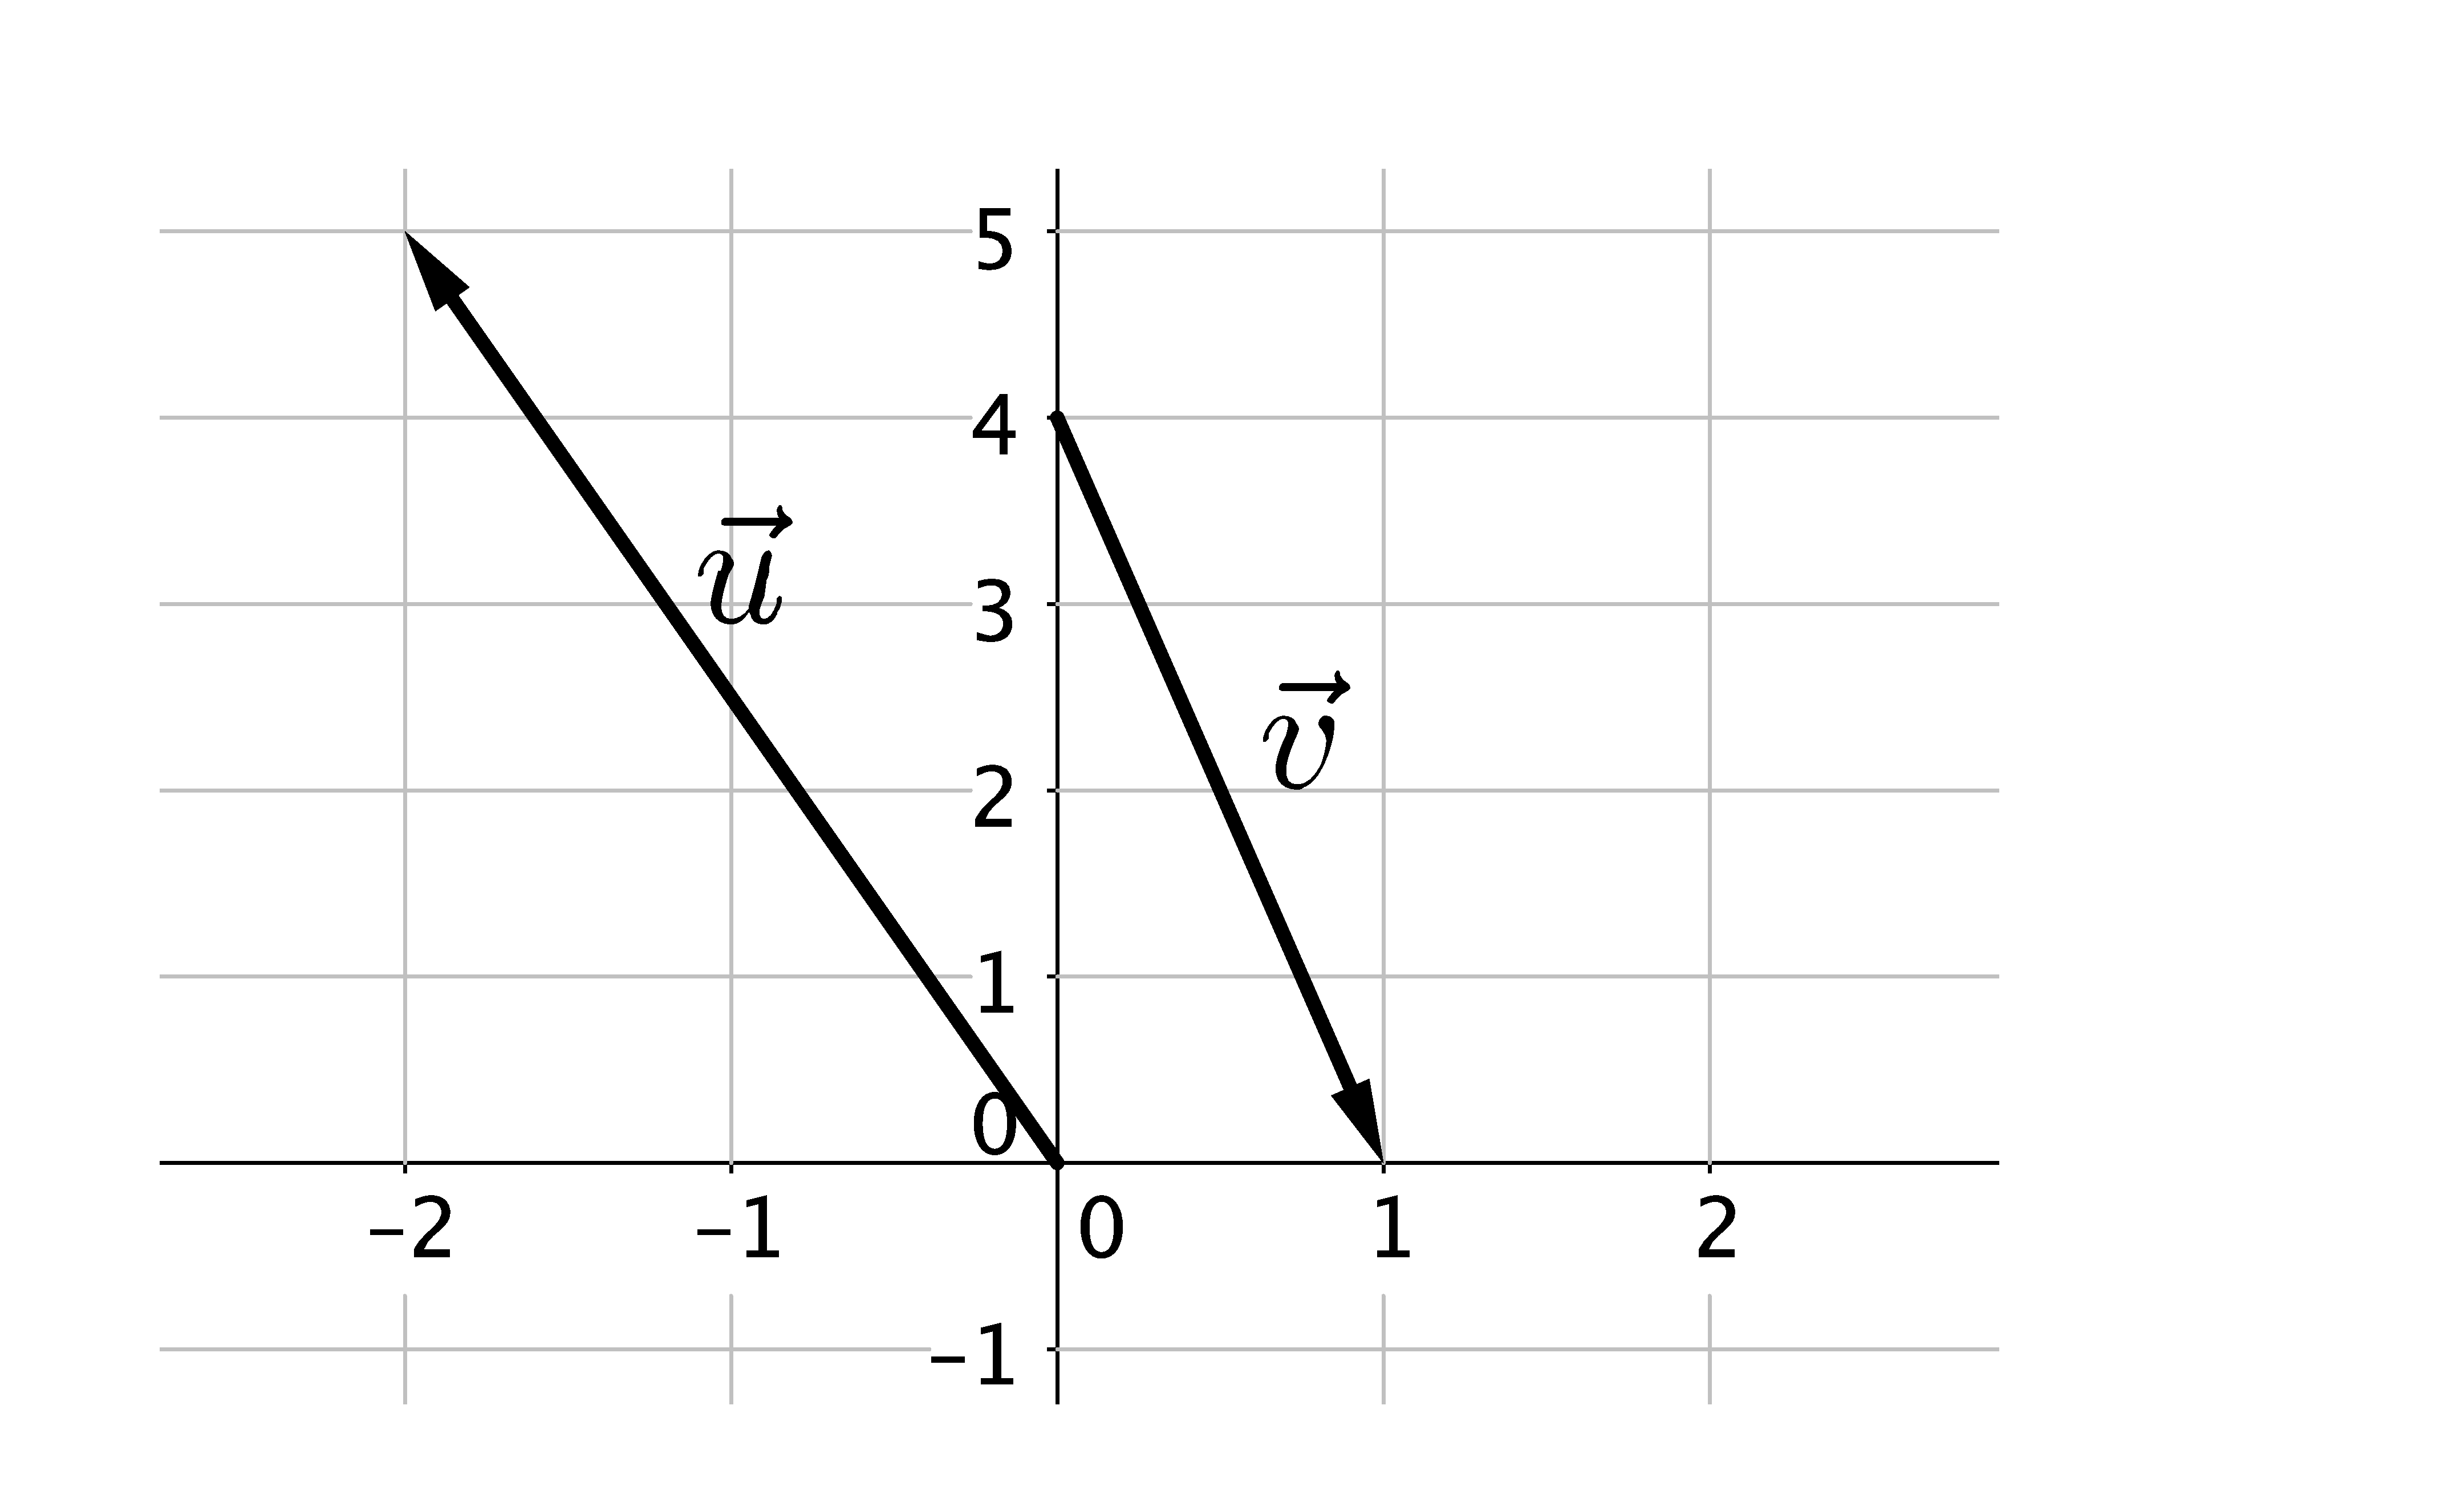
\includegraphics[width=0.6\textwidth]{img2/vec-opera}
		\end{center}
\end{minipage}
 
	\item Troba el vector $\vec x$ tal que $\vec a = 3 \vec b -\frac{1}{2} \vec x$, essent $\vec a=(7,-2)$ i $\vec b =(-1,3)$.
	
\end{mylist}

\hot Pàg. 35. Ex. 1
  
 
 %%%%%%%%%%%%%%%%%%%%%%%%%%%%%%%%%%%%%%%%%%%%%%%%%%%%%%%%%%%%%%%%%%%%%%%%%%%%%%%%%%%%%%%%%%%%%%%%%%%%%%%%%%%%%%%%%%%%%%%%%%%%%%%%%%%%%%%%%%%%%%%%
 \section{Bases i components}
 
 
 
 \begin{theorybox}[Dependència lineal]
 	Dos vectors $\vec u$, $\vvec$ són \textbf{linealment dependents} si tenen la mateixa direcció. Això passa si existeix un escalar $\lambda$ tal que $\vec u = \lambda \vvec$. Podem trobar una condició més pràctica en termes de les seves components, 
 	
  	$\dfrac{u_x}{\vx} = \dfrac{u_y}{\vy}$. Diem que les components han d'ésser proporcionals.
 	
 	Dos vectors $\vec u$, $\vvec$ són \textbf{linealment independents} si tenen la diferent direcció. 
 \end{theorybox}
 
  
 
 \begin{theorybox}[Definició de base]
 	Dos vectors $\vec u$, $\vvec$ són  \textbf{una base} del pla si: 
 	\begin{enumerate}
 		\item Són linealment independents
 		\item Tot vector $\vec w$, es pot expressar com combinació lineal dels altres dos $\vec w = \lambda \vec u + \mu \vvec$. Al parell de nombres $(\lambda, \mu)$ s'anomenen components del vector $\vec w$ respecte de la base $\mathcal{B}\{\vec u, \vvec\}$.
 	\end{enumerate} 
 \end{theorybox}
 
 \begin{resolt}{Troba les components del vector $\vec w(-3,-8)$ respecte la base formada pels vectors $\vec a(1,-3)$ i $\vec b(5,2)$}
 	
 	Es tracta d'expressar el vector $\vec w$ com a combinació lineal dels vectors de la base:
 	\begin{equation*}
 	\vec w = m \vec a + n \vec b
 	\end{equation*}
 	Substituïnt les components
 	
 	$(-3,-8)=m(1,-3)+n(5,2)$
 	
 	$(-3,-8)=(m,-3m)+(5n,2n)$
 	
 	$(-3,-8)=(m+5n,-3m+2n)$
 	
 	Igualam component a component i trobam el sistema d'equacions
 	
 	$\left\{\begin{array}{lll}
 	m &+5n &=-3 \\
 	-3m&+2n&=-8
 	\end{array}\right.$
 	Resolent el sistema anterior, arribam \linebreak a $m=2$, $n=-1$. Les components del vector $\vec w$ són $(2,-1)$.
 \end{resolt}
 
 \begin{mylist}
 	\item Determina si són dependents o independents les següents parelles de vectors:
 	\begin{tasks}(3)
 		\task $\vec u \left(2, \frac{2}{5} \right)$	i 	 $\vec v(-10,-9)$
 		\task $\vec u \left(-2, 3\right)$	i 	 $\vec v(-3, 2)$
 		\task $\vec u \left(-6, 9 \right)$	i 	 $\vec v(8, -12)$
 	\end{tasks}
 	
 	\item Què ha de valer $k$ perquè els vectors $\vec u(18, -6)$ i $\vvec(k, 4)$ tinguin igual direcció?
 \end{mylist}
  
 \begin{theorybox}[Base ortonormal o canònica]
 	Si prenem com a vectors $\vec i = (1, 0)$, $\vec j = (0,1)$ es fàcil comprovar que formen una base. Aquesta base s'anomena la base canònica o ortonormal. Ortonormal significa que els vectors tenen mòdul 1 i formen un angle de $90^\circ$.
 	
 	D'aquesta forma qualsevol vector $\vec w = (-5, 2)$ es pot expressar com $\vec w = -5 \vec i +  2\vec j$; és a dir $(-5, 2)$ són les components del vector $\vec w$ respecte de la base canònica.
 \end{theorybox}


 
 %%%%%%%%%%%%%%%%%%%%%%%%%%%%%%%%%%%%%%%%%%%%%%%%%%%%%%%%%%%%%%%%%%%%%%%%%%%%%%%%%%%%%%%%%%%%%%%%%%%%%%%%%%%%%%%%%%%%%%%%%%%%%%%%%%%%%%%%%%%%%%%%
 
 \section{Producte escalar}
 
 \begin{theorybox}[Definició]
 	Es defineix el producte escalar de dos vectors  $\vec u$, $\vvec$ com
 	\begin{equation}
 	\label{eq:dotproduct}
 	\vec u \cdot \vvec= |\vec u|\, |\vvec|\, \cos \alpha
 	\end{equation}
 	on $\alpha$ és l'angle que formen els vectors. \textbf{El producte escalar de dos vectors és un nombre.}
 	
 	Depenent de l'angle $\alpha$ tenim $\left\{ \begin{array}{ll} 
 	\alpha<90^\circ &   \vec u \cdot \vvec>0 \\ 
 	\alpha=90^\circ &   \vec u \cdot \vvec=0	\\
 	\alpha>90^\circ &  \vec u \cdot \vvec<0 
 	\end{array}\right.$
 	
 	Un resultat molt important és que dos vectors són \textbf{perpendiculars o ortogonals} si el seu \textbf{producte escalar és igual a zero}.		 
 \end{theorybox}
 
 \begin{mylist}
 	\item En una circumferència de centre O i de radi 2 cm, s'inscriu un hexàgon regular de vèrtexs $A, B, C, D, E, F$. Calcula els productes:
 	\begin{tasks}(4)
 		\task $\overrightarrow{OA}\cdot \overrightarrow{OB}$
 		\task $\overrightarrow{OA}\cdot \overrightarrow{OC}$ 
 		\task  $\overrightarrow{AB}\cdot \overrightarrow{ED}$
 		\task $\overrightarrow{BC}\cdot \overrightarrow{EF}$
 	\end{tasks}
 	
 \end{mylist}
 
 \begin{theorybox}[En base canònica]
 	Si disposam de les components  de $\vec u$, $\vvec$ respecte la base canònica
$\vec u \cdot \vvec= u_x \, \vx + u_y\, \vy$

 	Propietats del producte escalar:
 	\begin{enumerate}
 		\item Commutatiu: $\vec u \cdot \vvec = \vvec\cdot \vec u$
 		\item Distributiu 1: $\vec u \cdot (\vvec+ \vec w) = \vec u \cdot \vvec+ \vec u \cdot \vec w$	
 		\item Distributiu 2: $\vec u \cdot (\lambda \vvec) = \lambda (\vec u \cdot \vvec)$
 	\end{enumerate}
 \end{theorybox}
 
 \begin{resolt}[E]{Obté un vector ortogonal a $\vvec(8,6)$ i el mòdul del qual sigui igual a 4.}
 	El vector que cercam serà de la forma $(x,y)$ i ha d'ésser perpendicular a $\vvec$. Això passa si el producte escalar és igual a 0:
 	\begin{equation*}
 	(8,6)\cdot(x,y)=8x+6y=0
 	\end{equation*}
 	Una possible solució és $x=-6$ i $y=8$ però evidentment no té el mòdul adequat. 
 	
 	Aquest vector té mòdul  $|\vec x|=\sqrt{6^2+8^2}=10$. Això vol dir que el vector $\frac{1}{10}(-6,8)$ és unitari i, per tant,  $\frac{4}{10}(-6,8)=(-\frac{12}{5}, \frac{16}{5})$ tindrà mòdul 4.
 \end{resolt}

\hot Pàg. 35. Ex. 3

\begin{mylist}
		\item Donats $\vec u =(2,3)$, $\vvec (-3,1)$ i $\vec w(5,2)$, calcula:
	\begin{tasks}(4)
		\task $(3\vec u + 2 \vvec) \cdot \vec w$
		\task $\vec u \cdot \vec w - \vvec \cdot \vec w$
		\task $(\vec u \cdot \vvec)\vec w$
		\task $\vec u (\vvec\cdot \vvec)$
	\end{tasks}
	Indica en cada cas si el resultat de l'operació és un vector o un escalar.
	
 	
	\item Què ha de valer $k$ perquè els vectors $\vec u(18, -6)$ i $\vvec(k, 4)$ siguin perpendiculars?
\end{mylist}


 
 
 %%%%%%%%%%%%%%%%%%%%%%%%%%%%%%%%%%%%%%%%%%%%%%%%%%%%%%%%%%%%%%%%%%%%%%%%%%%%%%%%%%%%%%%%%%%%%%%%%%%%%%%%%%%%%%%%%%%%%%%%%%%%%%%%%%%%%%%%%%%%%%%%
 \section{Mòdul i angles}
 \begin{theorybox}
 	El mòdul d'un vector s'obté de l'equació (\ref{eq:dotproduct}) fent que $\vec u = \vvec$. Es compleix que $|\vvec| = \sqrt{\vvec \cdot \vvec}$ i si utilitzam la base canònica  $| \vvec |=\sqrt{\vx^2+\vy^2}$.
 	
 	Un vector és \textbf{unitari} si té mòdul 1. Per conseguir que un vector sigui unitari basta dividir-lo pel seu mòdul.
 	
 	L'angle que formen dos vectors s'obté aïllant-lo de l'equació  (\ref{eq:dotproduct}):
 	\begin{equation}
 	\label{eq:angle}
 	\alpha = \arccos \dfrac{\vec u \cdot \vvec}{|\vec u|\, |\vvec|} = \arccos \dfrac{ u_x \, \vx + u_y\, \vy }{\sqrt{u_x^2+u_y^2} \, \sqrt{\vx^2+\vy^2}} 
 	\end{equation}
 \end{theorybox}
  
 \begin{resolt}[E]{Calcula $k$ perquè els vectors $\vec u(1, k)$ i $\vvec(3,-2)$ \vspace{1em}
 		
 		\begin{enumerate}\setlength\itemsep{1em}
 			\item[a)] formin un angle de $90^\circ$
 			
 			
 			
 			\item[b)] tingin el mateix mòdul
 			
 			
 			\item[c)] formin un angle de $60^\circ$
 		\end{enumerate}	
 	}
 	\begin{enumerate} 
 		\item[a)] Els dos vectors formaran un angle de $90^\circ$ si són perpendiculars. Això passa si el seu producte escalar és igual a 0. $\vec u \cdot \vvec = (1, k) \cdot (3,-2) = 3-2k=0$, d'on deduim que $k=3/2$. 
 		
 		\item[b)] Perquè tinguin el mateix mòdul
 		\begin{equation*}
 		\sqrt{1+k^2} = \sqrt{9+4}
 		\end{equation*}
 		Elevam al quadrat, $1+k^2=13$ i d'aquí $k=\pm \sqrt{12}$
 		
 		
 		\item[c)] Perquè formin un angle de $60^\circ$ els dos vectors
 		\begin{equation*}
 		\cos 60^\circ = \frac{3-2k}{\sqrt{1+k^2}\sqrt{9+4}}
 		\end{equation*}
 		Si elevam al quadrat l'equació i multiplicam en creu trobam $13(1+k^2)=4(3-2k)^2$. Si resolem aquesta equació de segon grau trobam: $k\approx 0.494$ i $k\approx 15.51$
 	\end{enumerate}
 \end{resolt}
  \vspace{0.5cm}
  
 \hot Pàg.35 5a), 9, 10, 12, 15, 16
   \vspace{0.5cm}
   
 \hrule
 \textbf{Solucions:}
 \begin{multicols}{2}
\textbf{5.a)} $AB=3$, $BC=2.24$, $AC=1.41$, $\hat A=45$, $\hat B=26.57$, $\hat C=108.43$
 
\textbf{9.} $AC=\sqrt{8}$, $BD=\sqrt{32}$, $Area=8$
 
 \textbf{10.} $x=\pm \sqrt{3}/3$; unitari $(1/2, \sqrt{3}/2)$
 
\textbf{ 12.} $D(1,6)$,  $\widehat{ABC}=153.43$
 
 \textbf{15.} a) No perpendiculars, b) Sí, c) Sí, d) No independents
 
\textbf{ 16.} $(-4, 1)$ o paral·lels a ell.
 \end{multicols}
  

\end{document}